\documentclass[11pt]{article}

\marginparwidth 0.5in 
\oddsidemargin 0.25in 
\evensidemargin 0.25in 
\marginparsep 0.25in
\topmargin 0.25in 
\textwidth 6in \textheight 8 in

% pacote para exibicao de codigo fonte em python
\usepackage{minted}
\usepackage{graphicx}

\begin{document}
\author{Isabella de Albuquerque Ceravolo}
\title{Solving the graph coloring problem with VNS}
\maketitle

\section{Introduction}
The graph coloring problem is related with the minimum number of colors needed to coloring all vertices of a graph, respecting that two adjacent vertices will not be colored with the same color. In other words, we want to find its chromatic number. An approach to solve this problem using variable neighborhood search (VNS) starts coloring all vertices with a different color and proceed with the local search until there are no changes in the graph for K iterations (K is a value defined by the user). Then some perturbations are applied to the current solution in order to explore new neighborhoods. This process is repeated for T interactions (defined by the user). The next section will give more details about the algorithm developed and its implementation. The section \ref{test} presents some examples used to observe the algorithm's effectiveness.

\section{Algorithm description}
The algorithm is based on the VNS metaheuristic. There are basically two main actions: perform a local search to find a better solution and apply some disturbances in the current solution. Before this two steps, is crucial to define an initial strategy for coloring. In this algorithm, the starting point is to color differently all vertices of the graph. That is, a graph with N vertices begins with N colors. Thus, we start with a valid solution that may use more colors than necessary.

The neighborhood to be covered in local search may be obtained by randomly selecting a node in the graph G and coloring it with another color present in G. The new color is randomly selected among the colors in currently used in the graph (excluding the current color of the node and the colors of its neighbors). The colors are represented by integers to facilitate the implementation. When local search do not offer any new solution for K iterations, the current solution is disturbed. The disturbance is to select two nodes randomly and swap their colors. This change is done K times. The changes will not change the number of colors used in G and (in the worst case) may violate the restriction that neighboring nodes must have different colors. If we are lucky, violations will be undone by the local search. Anyway, a new solution will be able to replace the current solution only if it complies with the restrictions.

The algorithm was implemented using Python and some of its libraries. The following list presents the tools used in this work.
\begin{itemize}
    \item \textbf{PyPy 5.3.1}: In order to attain a better performance during the algorithm execution, an alternative Python interpreter was used. PyPy is recognized by its speed, efficiency and compatibility with the original CPython interpreter (Python 2.7); 
    \item \textbf{NetworkX 1.11}: This is a Python package for manipulate graphs and complex networks. It was used in order to simplify the graph representation in the program;
    \item \textbf{Graphviz 0.4.10}: This a library for graph visualization. It was used to provide the visual output to the program. To run the code developed in this work, is also required to install the Graphviz program. In Linux systems, it can be made by the command \textbf{\textit{\$ apt-get install graphviz}} .
\end{itemize}

All these libraries can be downloaded using \textbf{\textit{pip}}. The source code is available at Git repository\footnote{The repository URL is: https://github.com/iac-isabella/GraphColoringVNS}. For linux environments, it can be executed (with sudo privileges) through the command: \textbf{\textit{\$ pypy ./VNS.py}}

The program input data consists in:
\begin{itemize}
    \item The name of the text file containing the graph definition to be colored. This definition is made specifying an edge by line (indicating the nodes that it connects separated by a tab space);
    \item The value of K (used to control the application of disturbances);
    \item The value of T (number of interactions that will be  executed).
\end{itemize}

\section{Testing the algorithm}
\label{test}
In order to verify the effectiveness of the algorithm, the program was executed using three examples of graphs:
\begin{itemize}
    \item A graph with five nodes and four edges;
    \item A graph with ten nodes and eleven edges;
    \item A graph with fifteen nodes and  fourteen edges.
\end{itemize}

As result from the program execution, the best solution found is plotted as a PNG image. The images generated during the tests are presented bellow. The colors are represented by integers. The parameters used in the test can be summarized in the following table.
\begin{table}[ht]
\centering
\begin{tabular}{|c|c|c|}
\cline{1-3}
\textbf{Vertices} & \textbf{K} & \textbf{Interactions (T)} \\ \cline{1-3}
5                 & 5          & 10          \\ \cline{1-3}
10                & 5          & 30          \\ \cline{1-3}
15                & 5          & 60          \\ \cline{1-3}
\end{tabular}
\end{table}



\begin{figure}[!htb]
\centering
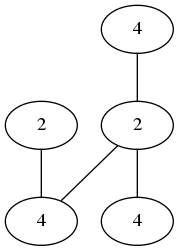
\includegraphics[scale=0.5]{a.png}
\caption{In the first test, the result uses the minimum number of colors.}
\end{figure}

\begin{figure}[!htb]
\centering
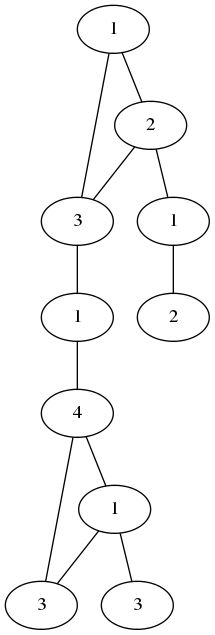
\includegraphics[scale=0.5]{b.png}
\caption{In the second test, the result uses one color more than the chromatic number.}
\end{figure}

\begin{figure}[!htb]
\centering
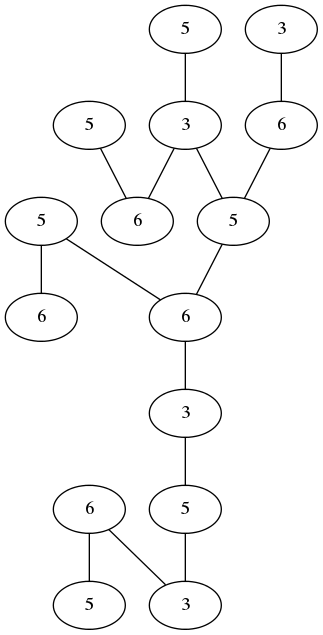
\includegraphics[scale=0.5]{c.png}
\caption{The last result also uses more colors than necessary.}
\end{figure}

%\begin{minted}[bgcolor=cyan!10]{python}
%# commments
%def func(asdf):
%    print "Hello"
%
%func("blabla")
%\end{minted}

\end{document}
